% Copyright 2020 by Junwei Wang <i.junwei.wang@gmail.com>
%
% This file may be distributed and/or modified under the
% conditions of the LaTeX Project Public License, either version 1.3c
% of this license or (at your option) any later version.
% The latest version of this license is in
%   http://www.latex-project.org/lppl.txt

\documentclass[compress]{beamer}

\usepackage[english]{babel}
\usepackage{metalogo}
\usepackage{listings}
\usepackage{fontspec}
\usepackage{tikz}

\usetheme{Nord}
% \usetheme[style=light]{Nord}

\setmainfont{Yanone Kaffeesatz}
\setsansfont{Andika New Basic}
\setmonofont{DejaVu Sans Mono}


\title{2016 GAISE College Report \\
        \large (Activity developed by Matthew Beckman)}
\author{Elle Butler and Elizabeth Eisenhauer}
\date{\today}

\begin{document}

\begin{frame}[plain,noframenumbering]
  \maketitle
\end{frame}

\section{Introductions}

\begin{frame}{Elizabeth (Liz) Eisenhauer}
\begin{itemize}
   \item Co-Advisors: Ephraim Hanks and Matt Beckman
   \item Research interests: animal movement modeling and statistics education
\end{itemize}

\begin{figure}
\centering
\begin{subfigure}
  \centering
  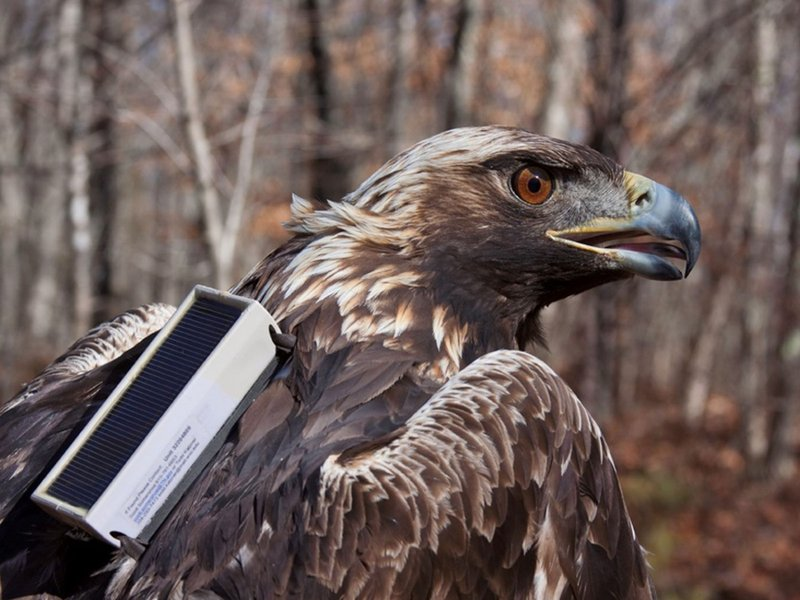
\includegraphics[width=.4\linewidth]{images/800.jpeg}
\end{subfigure}
\begin{subfigure}
  \centering
  
\includegraphics[width=.4\linewidth]{images/ed.jpeg}
\end{subfigure}
\end{figure}

\end{frame}

%-------------------

\begin{frame}{Elle Butler}
    
\end{frame}

%-----------------

\section{GAISE}

\begin{frame}{Guidelines for Assessment and Instruction in Statistics Education}{(GAISE)}
  \begin{enumerate}
    \item Teach statistical thinking  
    \begin{enumerate}
        \it{\item[A.] Teach statistics as an investigative process of problem solving and decision making}
        \item[B.] \it{Give students experience with multivariable thinking}
    \end{enumerate} 
    \item Focus on conceptual understanding
    \item Integrate real data with a context and purpose
    \item Foster active learning
    \item Use technology to explore concepts and analyze data
    \item Use assessments to improve and evaluate student learning
\end{enumerate}
\end{frame}

%------------------

\section{Discussion Acitivity}

\begin{frame}[fragile]{Group Assignments}
  \begin{itemize}
      \item \textbf{Group 1}: Guideline 1
      \item \textbf{Group 2}: Guidelines 2-4
      \item \textbf{Group 3}: Guidelines 5-6
  \end{itemize}

\end{frame}

%--------------------

\begin{frame}{Part I: Summarize your assigned GAISE guidelines}

Break out for 10 minutes.
\vspace{.5cm}

Be prepared to summarize each of your assigned GAISE guidelines for the class.  For example,
\begin{enumerate}
    \item Why is this important?
    \item What is this guideline intended to accomplish?
    \item What sort of examples did the authors of the GAISE College Report describe?
\end{enumerate}
    
\end{frame}

%-------------------

\begin{frame}{Part II: Action Plan}

Break out for 10 minutes.
\vspace{.5cm}

Prepare a specific plan to share with the class describing how an instructor could implement your assigned GAISE guidelines in: 

\begin{enumerate}
    \item A statistics course you are \textbf{currently taking} this semester 
    \item An \textbf{introductory statistics course} like STAT 200 at Penn State 
\end{enumerate}
We will critique these suggestions as a class to refine our thinking about the GAISE guidelines and help everyone begin to think about how they will incorporate GAISE guidelines into upcoming practice teaching assignments.
\end{frame}

% -----------------------

\begin{frame}{Part III: Topics Omitted from Introductory Statistics}

Break out for 10 minutes.
\vspace{.5cm}

Be prepared to share your remarks about the topics the might be omitted from introductory statistics courses.  

\begin{enumerate}
    \item Which topics are you glad to see on this list?
    \item Are there topics listed that you believe should \textbf{NOT} be excluded?
    \begin{enumerate}
        \item Share reasons why you'd like it to remain in the course
        \item Share reasons why it might reasonably be excluded
    \end{enumerate}
    \item Are there topics missing from the list that you think should be included?
    \begin{enumerate}
        \item Share reasons why you'd like it to be excluded
        \item Share reasons why it might reasonably remain in the course
    \end{enumerate}
\end{enumerate}
    
\end{frame}

\end{document}

%%% Local Variables:
%%% mode: latex
%%% TeX-master: t
%%% TeX-engine: xetex
%%% End:
